\documentclass{article}
\usepackage[UTF8]{ctex}
\usepackage[margin=0.7in]{geometry}
\usepackage{enumitem}
\usepackage{listings}
\usepackage{amsmath}
\usepackage{mathtools}
\usepackage{booktabs}
\newif\iffastbuild
\fastbuildtrue
\iffastbuild
    \usepackage[draft]{graphicx}
\else
    \usepackage{graphicx}
\fi
\usepackage{csvsimple}



\begin{document}

\begin{titlepage}
    \centering
    \vspace*{2cm}
    
    {\Huge\bfseries Building LLM Reasoners\par}
    \vspace{0.5cm}
    {\Large Assignment 2\par}
    \vspace{2cm}
    
    {\Large\bfseries Systems and Parallelism\par}
    \vspace{3cm}
    
    {\Large Siva Satvik\par}
    \vspace{0.5cm}
    {\large sm12779\par}
    \vspace{2cm}
    
    \vfill
\end{titlepage}

\begin{enumerate}[start=1,label=\arabic*.]
    \item \textbf{Profiling and Benchmarking}
    \begin{enumerate}
        \item[1.1.3] \textbf{\texttt{benchmarking\_script}}
            \begin{enumerate}[label=\alph*.]
                \item The script is present at student/benchmark.py
                \item The following table shows the timings for the forward and forward+backward passes for each of the model sizes (with context length as 256). The mean and standard deviation are computed across 10 runs for each model size and pass type.
                    \begin{table}[h]
                        \centering
                            \begin{tabular}{|r|r|r|r|}
                                \hline
                                model\_size & pass & mean\_step\_ms & std\_step\_ms \\
                                \hline
                                small & forward & 34.7421 & 0.2440 \\
                                \hline
                                small & forward+backward & 84.1578 & 0.4178 \\
                                \hline
                                medium & forward & 71.0755 & 3.2061  \\
                                \hline
                                medium & forward+backward & 215.5571 & 0.3645  \\
                                \hline
                                large & forward & 141.2933 & 0.1184 \\
                                \hline
                                large & forward+backward & 436.3411 & 0.3570  \\
                                \hline
                                xl & forward & 280.6156 & 0.0603 \\
                                \hline
                                xl & forward+backward & 888.9120 & 0.1919  \\
                                \hline
                                2.7B & forward & 417.7063 & 0.1057 \\
                                \hline
                                2.7B & forward+backward & 1320.3845 & 1.0714  \\
                                \hline
                            \end{tabular}
                    \end{table}
                    Backward pass is taking significantly more time than the forward pass, which is expected since it involves computing gradients for all parameters. As the model size increases, both forward and backward pass times increase, with the backward pass showing a more significant increase due to the larger number of parameters and computations involved. Generally, variance in timings is low (medium forward pass has higher variance than others), which suggests that the measurements are consistent across runs.
                \item When running the measurement steps without the warmup steps, the timings for the first couple of iterations are significantly higher than the subsequent iterations. This is obvious when running the measurement steps with 2 warmup steps, where the timings are almost same as runs with 5 warmup steps as in the previous experiment. This is because the first few iterations involve additional overhead from things like memory allocation, kernel compilation, and other setup tasks that are not representative of the steady-state performance of the model. By including warmup steps, we allow the system to reach a more stable state before we start measuring the performance, which results in more accurate and consistent timing measurements.
            \end{enumerate}
        \item[1.1.4] \textbf{\texttt{nsys\_profile}}
            \begin{enumerate}[label=\alph*.]
                \item The times for forward pass here are very similar to the times obtained in the previous section for the forward pass. This is expected since both measurements are for the same operation (forward pass) and should be consistent (The context length is the same in the comparision).
                \item The CUDA kernel that takes the most time in the forward pass is the ampere\_sgemm\_128x64\_tn kernel, which is a matrix multiplication kernel used in the transformer block. This kernel is responsible for Q, K, V and output matrix multiplications in attention layer and feed forward layers weights computations. Per transformer block, there are 7 calls to this kernel and for one forward pass, it will be number of blocks * 7 calls to this kernel. In both forward and backward pass, there's another kuda kernel that takes almost similar time as the ampere\_sgemm\_128x64\_tn kernel, which is the ampere\_sgemm\_128x128\_nt kernel. This kernel is also a matrix multiplication kernel used in the transformer block, and it is responsible for the matrix multiplications in the feed forward layers and attention output computations. The presence of these two kernels as the most time-consuming ones in both forward and backward passes indicates that matrix multiplication operations are the primary bottleneck in the performance of the transformer model.
                \item
                \item
                \item
            \end{enumerate}
        \item[1.1.5] \textbf{Mixed Precision}
            \begin{itemize}
                \item \textbf{\texttt{mixed\_precision\_accumulation\_test}}\\
                The output of the given code is as follows:
                    \begin{verbatim}
                        tensor(10.0001)
                        tensor(9.9531, dtype=torch.float16)
                        tensor(10.0021)
                        tensor(10.0021)
                    \end{verbatim}
                \textbf{Case 1: Pure Float32 Accumulation}
                In this scenario, both the accumulator and the increment use 32-bit single precision, which provides approximately 7 decimal digits of resolution. This is sufficient to represent the value 0.01 accurately enough that the final sum reaches 10.0001, showing nearly perfect alignment with the theoretical result.\\
                \textbf{Case 2: Pure Float16 Accumulation}
                Using 16-bit half precision significantly limits the available bits for the fraction, resulting in only about 3 decimal digits of precision. As the sum grows, the "gap" between representable numbers becomes larger than the 0.01 increment, causing the addition to lose precision or stall entirely, which leads to the inaccurate result of 9.9531.\\
                \textbf{Case 3: In-place Mixed Precision Addition}
                This case uses a Float32 sum but attempts to add a Float16 tensor directly to it, which triggers implicit type promotion. While the sum is more stable than Case 2, the increment itself was already "quantized" to a less accurate Float16 version of 0.01, resulting in a final sum (10.0021) that carries that initial approximation error through 1,000 steps.\\
                \textbf{Case 4: Explicit Float32 Casting}
                This implementation explicitly casts the Float16 increment to Float32 before performing the addition to ensure the operation occurs in a high-precision space. The result is identical to Case 3 (10.0021) because the bottleneck is the original creation of the value in Float16; once the precision is lost during the initial tensor creation, casting it to Float32 cannot recover the original ``perfect'' decimal value.\\
                \item \textbf{benchmarking\_mixed\_precision}
                    \begin{enumerate}[label=\alph*.]
                        \item The data types for each of the components is given below:
                            \begin{itemize}
                                \item the model parameters within the autocast context: \textbf{float32}
                                \item ToyModel.fc1: \textbf{float16}
                                \item ToyModel.ln: \textbf{float32} (Layer norm is kept in higher precision)
                                \item the models's predicted logits: \textbf{float16}
                                \item the loss: \textbf{float32} (loss is kept in higher precision for stability)
                                \item the model's gradients: \textbf{float32} (gradients are kept in higher precision for stability)
                            \end{itemize}
                        \item Layer normalization is sensitive in its reduction-heavy steps: computing mean/variance, subtracting the mean, squaring, and reciprocal square-root can lose stability in FP16 due to limited dynamic range and precision. BF16 has much larger exponent range (similar to FP32), so overflow/underflow risk is lower than FP16, but mantissa precision is still limited. In practice, many systems still keep LayerNorm in FP32 for robustness, though BF16 usually requires fewer special-case protections than FP16.
                        \item 
                        %For small model, the forward pass time with mixed-precision is slightly higher than the forward pass time with pure float32 precision. Whereas forward and backward pass times are similar for both pure float32 and mixed precision.\\ For medium model also, the forward pass time with mixed-precision is slightly higher than the forward pass time with pure float32 precision. However, forward and backward pass time with mixed precision is somewhat lower than that of pure float32. This could be because of larger computation being done in backward pass as the model size grows.\\ For large model, the forward pass time with mixed-precision is somewhat lower than the forward pass time with pure float32 precision. And forward and backward pass time with mixed precision is significantly lower than pure float32 precision. This is expected behaviour from the previous observation of difference between small and medium models.\\ For xl model, the forward pass time with mixed-precision is significantly lower than the forward pass time with pure float32 precision. And forward and backward pass time with mixed precision is significantly lower than pure float32 precision.\\ It's similar behavior for 2.7B model as well, where the forward pass time with mixed-precision is significantly lower than the forward pass time with pure float32 precision. And forward and backward pass time with mixed precision is significantly lower than pure float32 precision.\\
                        The forward pass times \textbf{started being same time or slightly higher for mixed precision in small model}, but as the model size increases, the \textbf{forward pass times for mixed precision become significantly lower than pure float32 precision}. This is because as the model size increases, the computational load increases and the benefits of using mixed precision (like faster computation and reduced memory bandwidth) become more pronounced, leading to greater performance improvements compared to pure float32 precision.
                        The below chart shows the forward+backward pass times for pure float32 and mixed precision across different model sizes (-bf16-mixed at the end refers to runs with mixed precision, and -fp32 at the end refers to runs with pure float32 precision):
                        \begin{center}
                            \includegraphics[width=0.8\textwidth]{../charts/mixed_precision_chart.png}
                        \end{center}
                    \end{enumerate}
            \end{itemize}
        \item [1.1.6] \textbf{memory\_profiling}
            \begin{enumerate}[label=\alph*.]
                \item The following two images are the memory profiles for the forward pass and the full training step (forward+backward+optimizer) for the large model at context length 512. The memory usage is significantly higher for the full training step compared to the forward pass alone, which is expected since the backward pass and optimizer steps require additional memory for storing gradients and optimizer states. The peaks in memory usage correspond to the points in the computation where large intermediate tensors are created, such as during matrix multiplications in the transformer blocks. The memory profile also shows that the memory usage is relatively stable during the forward pass, while it fluctuates more during the full training step due to the additional computations and memory allocations involved in the backward pass and optimization steps.
                    \begin{center}
                        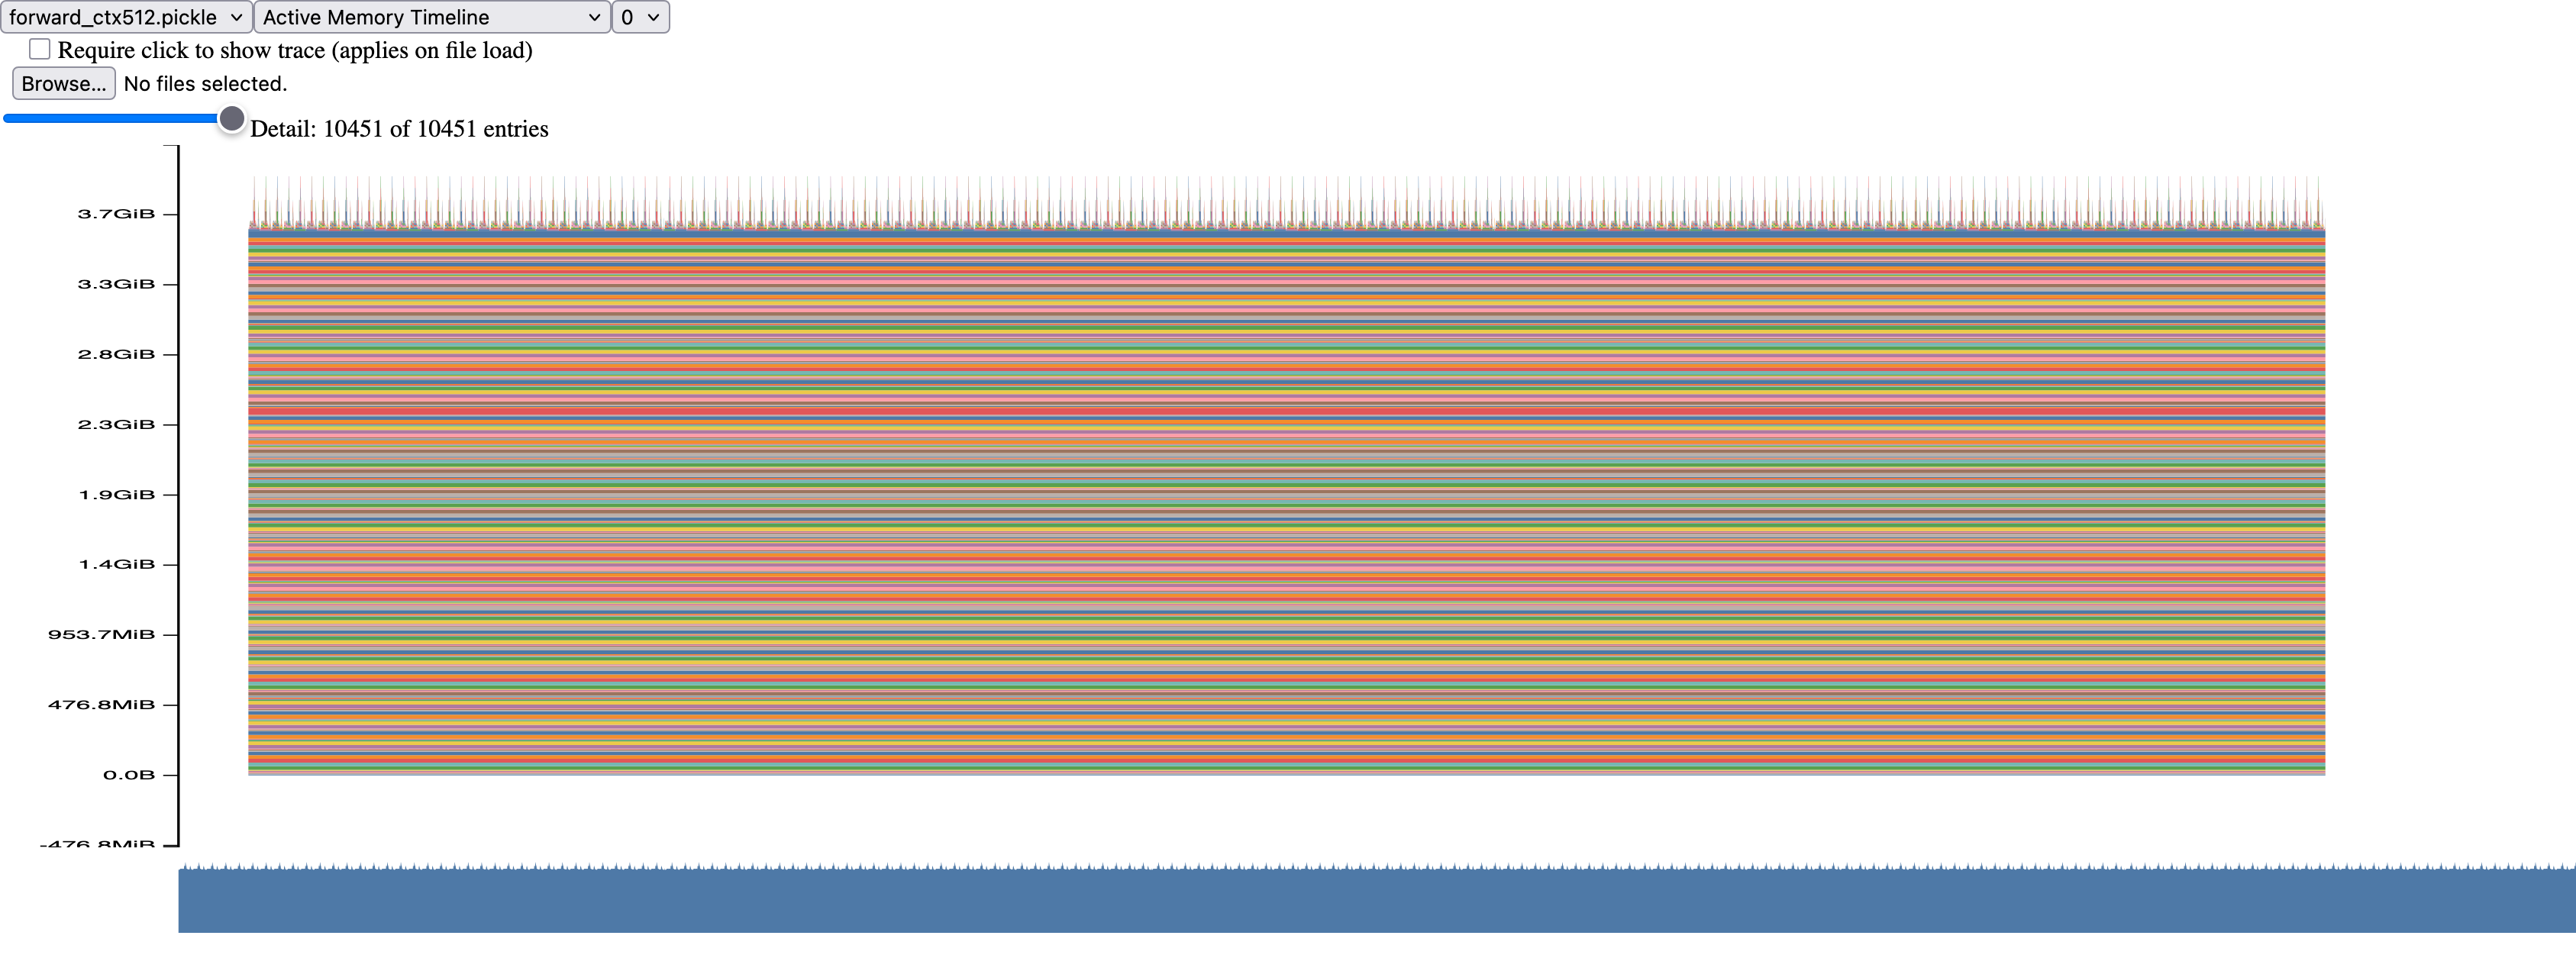
\includegraphics[width=0.8\textwidth]{../charts/large_forward_pass_memory_profile.png}
                    \end{center}
                    \begin{center}
                        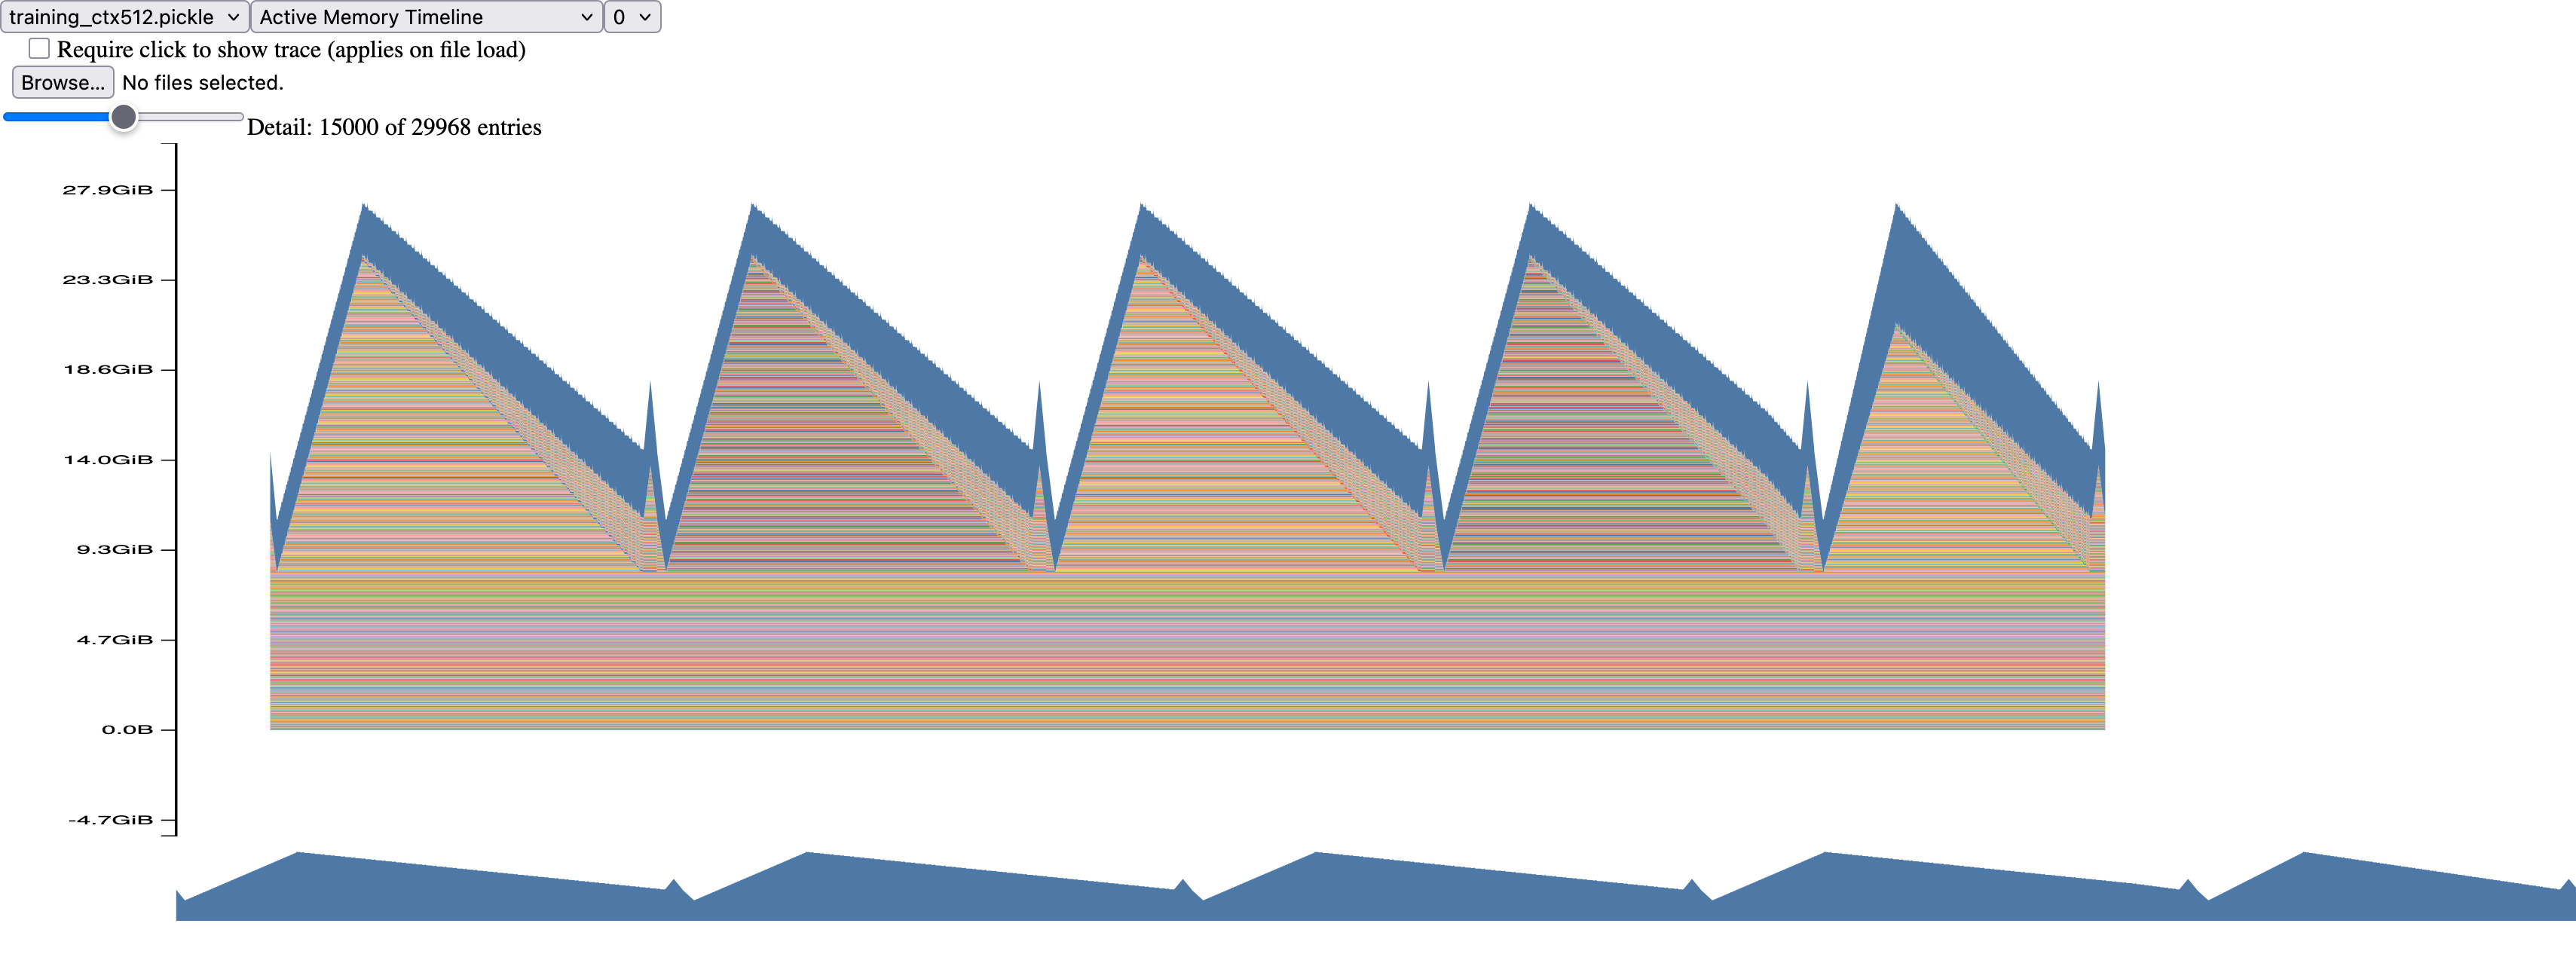
\includegraphics[width=0.8\textwidth]{../charts/large_full_training_step_memory_profile.png}
                    \end{center}
                \item Peak memory usage table is given below
                    \begin{table}[h]
                        \centering
                            \begin{tabular}{|r|r|r|}
                                \hline
                                context\_length & Forward pass peak memory & Full Training step peak memory\\
                                \hline
                                128 & 3.7 GiB & 17.8 GiB \\
                                \hline
                                256 & 3.7 GiB & 18.1 GiB \\
                                \hline
                                512 & 4.0 GiB & 27.4 GiB \\
                                \hline
                            \end{tabular}
                    \end{table}
                \item Peak memory usage table for mixed precision is given below
                    \begin{table}[h]
                        \centering
                            \begin{tabular}{|r|r|r|}
                                \hline
                                context\_length & Forward pass peak memory & Full Training step peak memory\\
                                \hline
                                128 & 5.4 GiB & 18.1 GiB \\
                                \hline
                                256 & 5.4 GiB & 18.1 GiB \\
                                \hline
                                512 & 5.6 GiB & 23.7 GiB \\
                                \hline
                            \end{tabular}
                    \end{table}
                    \newline
                    The peak memory usage for the forward pass is higher in mixed precision compared to pure float32 precision. This is because in mixed precision, some tensors are stored in lower precision (like float16 or bfloat16) which can lead to increased memory fragmentation and overhead from storing additional metadata for managing different data types. However, the peak memory usage for the full training step is lower in mixed precision compared to pure float32 precision. This is because mixed precision allows for reduced memory bandwidth and faster computation, which can lead to more efficient use of memory during the backward pass and optimization steps, ultimately resulting in lower overall memory usage compared to pure float32 precision.
                \item The size of a tensor of activations in the Transformer residual stream, in single precision, for large model with context length 512 is around 80 MiB. This is calculated based on the dimensions of the tensor (batch size, sequence length, hidden size) and the data type (float32) used for storing the activations. The memory usage can be computed as: 
                    \begin{align*}
                        \text{Memory Usage} = \text{Batch Size} \times \text{Sequence Length} \times \text{Hidden Size} \times \text{Bytes per Element}
                    \end{align*}
                    For example, here the batch size is 4, sequence length is 512, hidden size is 1280, and each float32 element takes 4 bytes, the memory usage would be:
                    \begin{align*}
                        4 \times 512 \times 1280 \times 4 = 10,485,760 \text{ bytes} = \mathbf{10} \text{ MB}
                    \end{align*}
                \item For large model with context length 512, the size of the largest allocations during the forward pass is around \textbf{80 MiB}. Looking at the stacktrace, the allocation came from \texttt{scaled\_dot\_product \_attention} function, which is responsible for computing the attention scores and applying the attention mechanism in the transformer block. The large allocation is likely due to the need to store intermediate tensors for the attention computation, such as the query, key, value matrices and the resulting attention weights, which can be quite large given the dimensions of the model and the context length.
            \end{enumerate}
        \item [1.2.1] \textbf{pytorch\_attention}
            \begin{enumerate}[label=\alph*.]
                \item Attention scaling benchmark results are given below. The out of memory errors are seen for context length of 16384 across d\_model sizes. For d\_model size of 16 and context length of 16384, the memory for attention is around 16 GiB. This comes from the calculation of qkv, output and probability tensors. As the context length increases, the memory saved for backward pass increases significantly as seen in the table. To eliminate this memory cost, we can use techniques like gradient checkpointing, which allows us to recompute intermediate activations during the backward pass instead of storing them all in memory. This can significantly reduce memory usage at the cost of increased computation time during the backward pass. Another technique is to use mixed precision training, which can reduce the memory footprint of activations and gradients by using lower precision data types (like float16 or bfloat16) while still maintaining model performance.
                    \begin{table}[h]
                        \centering
                        \resizebox{\linewidth}{!}{%
                            \csvautobooktabular[respect underscore]{../benchmark_results/attention_scale_benchmark.csv}%
                        }
                    \end{table}
            \end{enumerate}
        \newpage
        \item [1.2.1] \textbf{pytorch\_compile}
            \begin{enumerate}[label=\alph*.]
                \item The table for uncompiled vs compiled version of attention is given below
                    \begin{table}[h]
                        \centering
                        \resizebox{\linewidth}{!}{%
                            \csvautobooktabular[respect underscore]{../benchmark_results/attention_scale_compile_comparison.csv}%
                        }
                    \end{table}
                \newpage
                \item The table for uncompiled vs compiled version of the model is given below. The forward pass times for the compiled version are somewhat lower than the uncompiled version across all model sizes. The forward+backward pass times for the compiled version are a somewhat higher than the uncompiled version for smaller models but they are somewhat lower as the model size increases, which is also expected since the optimizations from compilation can benefit both forward and backward computations. When optimizer step is also included, the run times are very close for both compiled and uncompiled versions across all model sizes, with the compiled version being slightly higher for smaller models and slightly lower for larger models. This could be because the optimizer step may not benefit as much from compilation optimizations as the forward and backward passes do. Overall, the performance difference between compiled and uncompiled versions is not very significant, but there is a trend of improved performance with compilation as the model size increases. For xl and 2.7B models, the run with optimizer step is giving oom errors, hence not included in the table.
                    \begin{table}[h]
                        \centering
                            \begin{tabular}{|r|r|r|r|r|}
                                \hline
                                implementation & model\_size & pass & mean\_step\_ms & std\_step\_ms \\
                                \hline
                                uncompiled & small & forward & 34.7421 & 0.2440 \\
                                \hline
                                compiled & small & forward & 30.6835 & 0.3930 \\
                                \hline
                                uncompiled & small & forward+backward & 84.1578 & 0.4178 \\
                                \hline
                                compiled & small & forward+backward & 86.9557 & 0.3059 \\
                                \hline
                                uncompiled & small & forward+backward+optimizer\_step & 93.0815 & 0.5335  \\
                                \hline
                                compiled & small & forward+backward+optimizer\_step & 95.7967 & 1.0436 \\
                                \hline
                                uncompiled & medium & forward & 71.0755 & 3.2061  \\
                                \hline
                                compiled & medium & forward & 62.1534 & 2.7001  \\
                                \hline
                                uncompiled & medium & forward+backward & 215.5571 & 0.3645  \\
                                \hline
                                compiled & medium & forward+backward & 220.9293 & 1.1892  \\
                                \hline
                                uncompiled & medium & forward+backward+optimizer\_step & 243.2726 & 0.6310  \\
                                \hline
                                compiled & medium & forward+backward+optimizer\_step & 244.3076 & 3.1609  \\
                                \hline
                                uncompiled & large & forward & 141.2933 & 0.1184 \\
                                \hline
                                compiled & large & forward & 128.7720 & 0.0764 \\
                                \hline
                                uncompiled & large & forward+backward & 436.3411 & 0.3570  \\
                                \hline
                                compiled & large & forward+backward & 416.8952 & 0.9826  \\
                                \hline
                                uncompiled & large & forward+backward+optimizer\_step & 498.9632 & 0.0770  \\
                                \hline
                                compiled & large & forward+backward+optimizer\_step & 479.9749 & 1.5860  \\
                                \hline
                                uncompiled & xl & forward & 280.6156 & 0.0603 \\
                                \hline
                                compiled & xl & forward & 260.4873 & 0.3039 \\
                                \hline
                                uncompiled & xl & forward+backward & 888.9120 & 0.1919  \\
                                \hline
                                compiled & xl & forward+backward & 829.2161 & 0.1592  \\
                                \hline
                                uncompiled & 2.7B & forward & 417.7063 & 0.1057 \\
                                \hline
                                compiled & 2.7B & forward & 398.7467 & 0.0683 \\
                                \hline
                                uncompiled & 2.7B & forward+backward & 1320.3845 & 1.0714  \\
                                \hline
                                compiled & 2.7B & forward+backward & 1263.8836 & 0.3676  \\
                                \hline
                            \end{tabular}
                    \end{table}
            \end{enumerate}
    \end{enumerate} 
\end{enumerate}

\end{document}